 \documentclass[11pt]{extarticle}
\usepackage{manualdoprofessor}
\usepackage{fichatecnica}
\usepackage{lipsum,media9}
\usepackage[justification=raggedright]{caption}
\usepackage[one]{bncc}
\usepackage[acorde]{../edlab}
\usepackage{marginnote}
\usepackage{pdfpages}
\usepackage[printwatermark]{xwatermark}
% \newwatermark[pagex=2]{
\includegraphics[scale=3.3]{watermarks/test-a.png}}	% página específica
% %\newwatermark[oddpages]{
\includegraphics{watermarks/test-a.png}}			% páginas ímpars
% %\newwatermark[evenpages]{
\includegraphics{watermarks/test-a.png}}			% págimas pares
% \newwatermark[allpages]{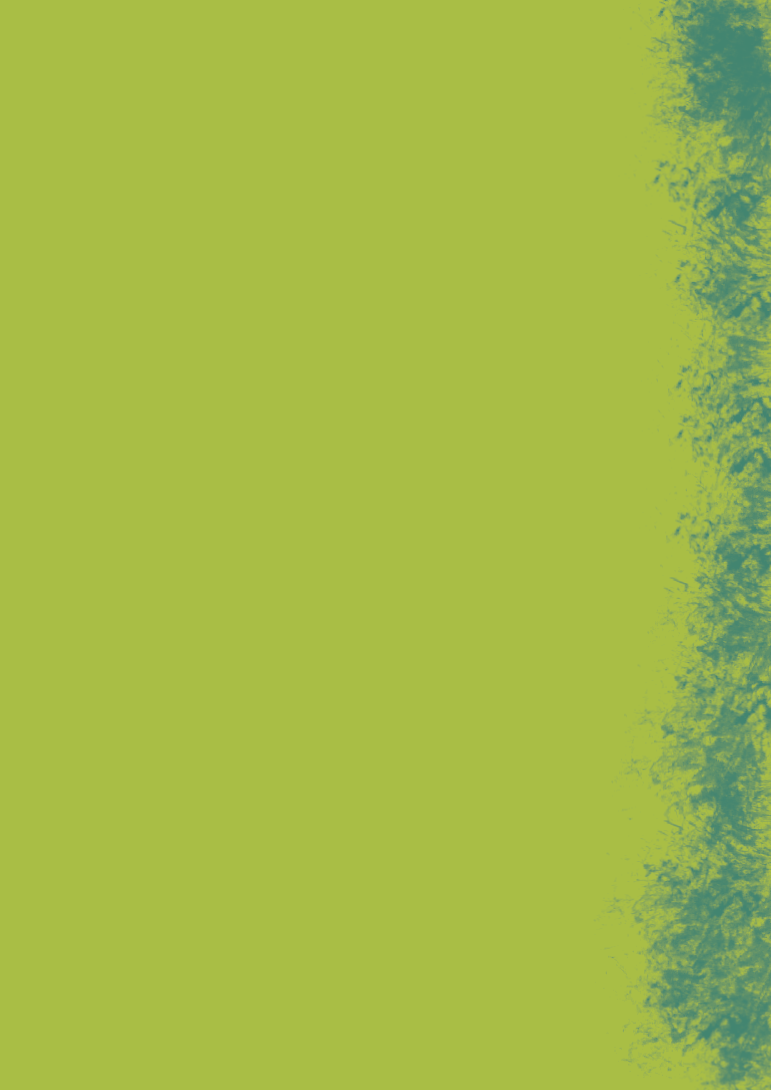
\includegraphics[scale=3.3]{watermarks/test-b.png}}

% \pagecolor{cyan!0!magenta!10!yellow!28!black!28!}

\newcommand{\AutorLivro}{Márcio Araújo}
\newcommand{\TituloLivro}{Figurinha Carimbada}
\newcommand{\Genero}{Conto}
%\newcommand{\imagemCapa}{./images/PNLD0001-01.png}
\newcommand{\issnppub}{978-65-99441-24-0}
\newcommand{\issnepub}{978-65-99441-27-1}
% \newcommand{\fichacatalografica}{PNLD0001-00.png}
\newcommand{\colaborador}{Gabriela Karam}

\begin{document}

\title{\TituloLivro}
\author{\AutorLivro}
\def\authornotes{\colaborador}

\date{}
\maketitle

%\begin{abstract}\addcontentsline{toc}{section}{Carta ao professor}
%\pagebreak

\tableofcontents

\section{Carta ao professor}

Caras e caros professores,

Este material tem a intenção de contribuir para que você consiga desenvolver um trabalho aprofundado com a obra \textit{Figurinha carimbada}, assim como auxiliar em jogos para que torne o aprofundamento da leitura mais lúdico e divertido. Contamos com vocês para mergulharmos juntos nessa história de seis meninos que compartilham mais ou menos as mesmas idades dos estudantes os quais vocês acompanham e que provavelmente passam pelas mesmas angústias, medos e dificuldades emocionais para se relacionarem com os colegas e o mundo ao redor. Não é à toa que \textit{Márcio Araújo}, o autor, escolhe a frase de Clarice Lispector, uma das maiores escritoras dos últimos tempos: viver dói. Para dar início a essas aventuras cotidianas que vagueiam pelas páginas do seu livro através das histórias de seis meninos na fase da pré adolescência, Araújo divide como que em capítulos o seu livro, com os nomes dos protagonistas de cada história e segue em primeira pessoa com maestria, sem ter medo de se misturar ou confundir os leitores, que conseguem distinguir cada um deles com muita exatidão. As histórias de Cauê, Guilherme, Luiz Felipe, Marquinhos, João e Ícaro nem sempre se cruzam diretamente, mas as angústias dos meninos se relacionam de uma forma ou outra. Cada uma delas carrega emoções muito profundas que certamente ajudarão em uma identificação com momentos em que as crianças estão passando ou mesmo já passaram. Um livro para ser lido e relido para não esquecermos nunca a criança que fomos e ainda somos.

As histórias são contadas com a atmosfera de diário, algo que pode servir de inpiração para que as crianças passem a escrever mais sobre suas questões e aprendam a externalizar sentimentos que muitas vezes os atravessam, mas não são verbalizados e nem colocados no papel. Além disso, situações que permeiam a vida das crianças são colocadas em pauta, como o termo "esquisito", corriqueiramente usado para depreciar pessoas que não estão dentro de alguns padrões e acaba sendo objeto para \textit{bullying}. No livro, o termo é utilizado por algumas das personagens para falarem de si mesmos e de seus amigos, desmistificando o termo e mostrando que estar fora desses padrões pode não ser um problema. Os meninos apresentam suas fragilidades e sensações ao longo de sua vivência na escola e mesmo em suas casas. Essas trajetórias são fundamentais para mostrar aos estudantes que cada pessoa tem sua subjetividade e sua vivência, uma vez que faz com que a turma entenda que as pessoas têm suas questões e sentimentos para lidar, e se abrir para fazer amizades é um passo muito importante para se relacionar com o mundo.

A literatura tem um poder muito forte de mostrar às pessoas que existem muitas formas de pensar a vida, muitas histórias diferentes e diversidade em inúmeros sentidos. Em \textit{Figurinha carimbada}, esse papel fundamental da literatura é ponto central, já que as crianças entram em contato com subjetividades que possivelmente nunca vieram à tona em suas vidas. Além disso, a obra promove uma infinidade de atividades das quais a turma poderá desfrutar, além de crescer muito e se divertir. Esperamos que gostem da variedade de atividades que apresentaremos no presente manual!

\Image{A literatura tem um poder muito forte de mostrar às pessoas que existem muitas formas de pensar a vida (Mercado Livros; Domínio público)}{PNLD2023-021-02.png}

\section{Sobre o livro}

Os contos presentes em \textit{Figurinha carimbada} mostram a vida de seis meninos que narram, em primeira pessoa, suas angústias, sonhos e emoções. De maneira aprofundada, a obra traz à tona as questões infantis que as crianças que não se enquadram nos padrões fixos da sociedade sofrem. O livro começa contando a história de Cauê, uma criança que não tem muitos amigos por ser tachado como uma pessoa esquisita, e mostra o início de uma amizade muito especial para ele. Seu grande amigo, Caio, acaba tendo que se mudar de cidade por questões familiares, e Cauê vive esse sofrimento, dialogando com o leitor sobre suas questões. A segunda história é de GuilheRme, um garoto que vive no interior. A personagem nos conta o percurso até perder seu cachorro, Tór, e abre seu coração para o leitor, mostrando como lida com a frustração da perda. O interessante é que Caio, o amigo de Cauê, agora está morando na mesma cidade de GuilheRme, e aparece na narrativa. No terceiro conto, conhecemos Luiz Felipe, personagem que nos mostra, por meio da literatura, que a lógica da produtividade não promove a felicidade, ao contrário: promove ansiedade e pouca vivência com presença. Além disso, a história de Luiz Felipe é atravessada pela questão de classes sociais e do racismo, uma vez que Luiz perde uma competição para o filho de Rosa, a faxineira e cozinheira que trabalha em sua casa, um garoto negro. E a absorção desse acontecimento é difícil para ele, até que a situação é resolvida. Ao longo da obra nos deparamos com diversas figuras que trazem, aos poucos, reflexões muito ricas.

\Image{O livro começa contando a história de Cauê (Falarcao; Domínio público)}{PNLD2023-021-03.png}

\section{Sobre o autor}

Márcio Araújo é um ator, autor, roteirista e diretor brasileiro. Entre seus trabalhos estão textos para mais de 500 episódios do Cocoricó da TV Cultura. Participa do grupo de teatro Pocilgas e Cia. Escreveu e dirigiu o Musical "Nara" sobre a vida da cantora Nara Leão, com Fernanda Couto. O musical ganhou o Prêmio Contigo!

\Image{Márcio Araújo é um ator, autor, roteirista e diretor brasileiro (Marcio Araújo; Domínio público)}{PNLD2023-021-04.png}

\section{Sobre o gênero}

O presente livro se trata de um \textbf{conto}, que é uma história curta, com poucos personagens e centrada em apenas um núcleo narrativo. Geralmente, o conto tem elementos lúdicos e utiliza expressões metafóricas, com o intuito de retratar o cotidiano de maneira poética e subjetiva. O texto também possui características da fábula. A fábula veio do conto, mas se diferencia pela centralidade de personagens animais e pelo intuito de concluir a história com um ensinamento moral.

\section{Proposta de Atividades}
\subsection{Pré Leitura}

A seguir você encontrará a descrição de uma aula modelo como exemplo prático para a exploração do livro com os estudantes. Esta seção apresentará orientações sobre como organizar a sala de aula para receber os estudantes, exercitar a interação entre eles e prepará-los para que o momento da leitura tenha mais riqueza de conteúdo. Antes que a leitura comece, é interessante aquecermos a turma e deixá-la com a sensibilidade mais inspirada. Dessa forma, eles terão mais recursos para absorver a obra com mais abundância.

\BNCC{EF35LP07}% Utilizar, ao produzir um texto, conhecimentos linguísticos e gramaticais, tais como ortografia, regras básicas de concordância nominal e verbal, pontuação (ponto final, ponto de exclamação, ponto de interrogação, vírgulas em enumerações) e pontuação do discurso direto, quando for o caso.
\BNCC{EF03LP07} %Identificar a função na leitura e usar na escrita ponto final, ponto de interrogação, ponto de exclamação e, em diálogos(discurso direto), dois-pontos e travessão.
\BNCC{EF05LP26}% Utilizar, ao produzir o texto, conhecimentos linguísticos e gramaticais: regras sintáticas de concordância nominal e verbal, convenções de escrita de citações, pontuação (ponto final, dois-pontos, vírgulas em enumerações) e regras ortográficas.
\BNCC{EF15AR01}%Identificar e apreciar formas distintas das artes visuais tradicionais e contemporâneas, cultivando a percepção, o imaginário, a capacidade de simbolizar e o repertório imagético.}
\BNCC{EF15LP18}%Relacionar texto com ilustrações e outros recursos gráficos.}

\paragraph{Tema} Redação. 

\paragraph{Conteúdo} Descrição subjetiva. 

\paragraph{Objetivo} Estimular o exercício criativo da redação por meio de uma descrição de um objeto. Preparar o aluno para os temas explorados em \textit{Figurinha carimbada}. 

\paragraph{Justificativa} A redação é uma forma de expressão da própria identidade e da manutenção da autoestima elevada.  

\paragraph{Metodologia} O professor pode pedir que cada estudante traga um objeto que o represente, alguma coisa que goste muito ou que tenha participação ativa na sua vida. Na próxima aula, já com os objetos, estimule que cada um conte uma história sobre esse objeto e a importância dele em sua vida. Em seguida, o educador os instrui a escrever, em uma página, o que acabaram de contar, colocando os seus nomes no final. Peça que eles reparem em sua escrita, provocando-os a estarem atentos às concordâncias nominal e verbal e à pontuação adequada para seus textos. Segue exemplo abaixo:

\textit{Eu trouxe um chaveiro de filtro de barro porque, quando mudaram para filtro de barro na minha casa, fiquei muito triste, achava o gosto da água muito esquisito. Minha mãe dizia que com o tempo esse gosto ia passar, mas eu não acreditava. Até que passou. E hoje, lá de casa eu sou a pessoa que mais gosta da água do filtro de barro, porque ela é fresquinha! Então um dia a gente tava na praia e meu pai viu um moço vendendo esse chaveiro e comprou pra mim.
Eva}

Depois que cada aluno tiver sua história escrita, sugira que eles façam um desenho que represente essa história. Para o desenho, estimule-os a trabalhar com os materiais disponíveis na escola: lápis, tinta, papéis, diferentes texturas. Depois disso, guarde todos os desenhos juntos. Coloque cinco objetos deles na frente da sala e conduza para que cinco alunos se aproximem de cada objeto, não podendo ser o seu. Logo após, entregue a eles os textos de cada objeto correspondente e peça para que leiam como se fossem seus objetos. Inclusive, ao invés de ler o nome que está escrito, falar o próprio nome da criança que está lendo para trazer intimidade na leitura do texto de outra pessoa. A dinâmica tem potencial para fazer com que a turma experimente ouvir um pouco a respeito da história de seus colegas e para que possam externalizar intimidades e trocar com seus colegas. 

\paragraph{Tempo Estimado} Quatro aulas de 50 minutos.

\Image{Depois que cada aluno tiver sua história escrita, sugira que eles façam um desenho que represente essa história (Rede estadual da Bahia; Domínio público)}{PNLD2023-021-05.png}

\subsection{Leitura}

\BNCC{EF03LP12}%Ler e compreender, com autonomia, cartas pessoais e diários, com expressão de sentimentos e opiniões, dentre outros gêneros do campo da vida cotidiana, de acordo com as convenções do gênero carta e considerando a situação comunicativa e o tema/assunto do texto.
\BNCC{EF15LP03}%Localizar informações explícitas em textos.
\BNCC{EF15LP09}% Expressar-se em situações de intercâmbio oral com clareza, preocupando-se em ser compreendido pelo interlocutor e usando a palavra com tom de voz audível, boa articulação e ritmo adequado.
\BNCC{EF15LP10} %Escutar, com atenção, falas de professores e colegas, formulando perguntas pertinentes ao tema e solicitando esclarecimentos sempre que necessário.

\paragraph{Tema} Leitura e compreensão de \textit{Figurinha carimbada}.

\paragraph{Conteúdo} Estrutura de \textit{Figurinha carimbada}: enredo, personagens, tempo, espaço e foco narrativo.  

\paragraph{Objetivo} Ler e compreender os contos de \textit{Figurinha carimbada} e sua estrutura. Promover o gosto pelos livros e pela leitura, estimular o desenvolvimento da linguagem e da criatividade.   

\paragraph{Justificativa} O professor tem grande influência na formação de leitores. É preciso fazer a mediação entre a obra, sua linguagem, suas estruturas, seus pressupostos e os estudantes, de preferência estabelecendo uma relação fundamentada no prazer, na identificação e na liberdade de interpretação. Eis o nosso desafio: ler com os alunos, apresentando as passagens decisivas de um texto, explicando por que elas chamam a atenção e  ouvindo as impressões dos estudantes a respeito de tudo isso. 

A escolha da narrativa feita pelo autor Márcio Araújo foi a divisão de cada capítulo pelo nome do protagonista, que contou a sua história em primeira pessoa de uma forma bem fluida. Cada história contada pela personagem principal de cada capítulo retrata de forma muito sensível determinado momento da vida que a criança estava passando. Para realizar essa leitura de uma forma agradável e que não gere um desconforto pra quem está lendo, sugere-se que as carteiras estejam da mesma forma como se posicionam numa sala de aula. O educador pode escolher seis alunas e alunos para lerem do seu próprio lugar a sua parte e sugerir que os outras fechem os olhos para absorver mais a história. Após a leitura, peça que cada pessoa escreva o nome de uma personagem que ela ou ele mais gostou e divida em grupos pelos nomes escolhidos. É sugerido que os estudantes sejam divididos nos grupos das personagens, divida-os entre os capítulos para que revezem a leitura. Depois de cada capítulo, peça que eles desenhem num papel um objeto que elas e eles achem que representa essa personagem pela história contada. Findada a leitura, faça uma exposição de cada grupo, mostrando e colando o desenho na frente da sala e pedindo que eles expliquem o motivo da escolha desse objeto com clareza e falem sobre o que acham que a personagem sentiria pelo objeto. Deixe que os alunos usem a imaginação e a criatividade, abrindo a possibilidade de, inclusive, mostrarem os motivos pelos quais se identificam com as personagens. Através dessa leitura conjunta, objetiva-se despertar o interesse do aluno pela identificação com a obra e as crianças que aparecem abrindo seus sentimentos no livro. No final de cada apresentação, deixe que a turma se envolva fazendo perguntas para os colegas, observações sobre as escolhas das crianças e comentando a atividade, sempre relacionando à experiência da leitura. 

\Image{A escolha da narrativa feita pelo autor Márcio Araújo foi a divisão de cada capítulo pelo nome do protagonista (Coc; Domínio público)}{PNLD2023-021-06.png}

Por fim, pode-se explorar mais detidamente os elementos do enredo. Fale sobre os diferentes momentos que o compõem:

\begin{enumerate}


\item A introdução das personagens;
\item Os sentimentos presentes em cada vida que se apresenta;
\item A sensação de exclusão;
\item A importância da socialização com amigos;
\item As fragilidades que uma criança pode enfrentar ao longo de sua vida. 


\end{enumerate}

\paragraph{Tempo Estimado} Quatro aulas de 50 minutos.

\Image{Fale sobre os diferentes momentos que o compõem (André Bets; Domínio público)}{PNLD2023-027-07.png}

\subsection{Pós-leitura}

\BNCC{EF35LP07}% Utilizar, ao produzir um texto, conhecimentos linguísticos e gramaticais, tais como ortografia, regras básicas de concordância nominal e verbal, pontuação (ponto final, ponto de exclamação, ponto de interrogação, vírgulas em enumerações) e pontuação do discurso direto, quando for o caso.
\BNCC{EF04LP05}% Identificar a função na leitura e usar, adequadamente, na escrita ponto final, de interrogação, de exclamação, dois-pontos e travessão em diálogos (discurso direto), vírgula em enumerações e em separação de vocativo e de aposto.}
\BNCC{EF04LP06}% Identificar em textos e usar na produção textual a concordância entre substantivo ou pronome pessoal e verbo (concordância verbal).}
\BNCC{EF03LP13} %Planejar e produzir cartas pessoais e diários, com expressão de sentimentos e opiniões, dentre outros gêneros do campo da vida cotidiana, de acordo com as convenções dos gêneros carta e diário e considerando a situação comunicativa e o tema/assunto do texto.

\paragraph{Tema} Carta. 

\paragraph{Conteúdo} Redação de carta.

\paragraph{Objetivo} Verificar a compreensão da leitura do livro, de forma criativa. 

\paragraph{Justificativa} Enquanto as atividades de leitura, compreensão e análise caracterizam-se pelas primeiras aproximações do texto, seguidas de atividades de descrição de suas características, a prática de redação abre espaço para que os estudantes criem suas próprias narrativas. 

Após a leitura, é interessante promover uma conversa sobre todas as histórias no geral, pedindo que os estudantes identifiquem quais personagens, de cada capítulo, estão ligados e qual é a relação que há entre eles. Peça que eles tragam informações detalhadas para verificar o entendimento do livro como um todo. Depois que esse momento de discussão acontecer, sugere-se que o professor peça que eles redijam uma carta para alguma das personagens, contando de sua vida e seus anseios do momento. Incentive-os a trazerem elementos que foram vistos no texto para incluir, na carta, a subjetividade da personagem escolhida também. Ao longo da escrita dos alunos, passe nas mesas sanando possíveis dúvidas e corrigindo individualmente os erros gramaticais, explicando os motivos dos erros e, quando houver recorrência de um erro específico, ir até a lousa e retomar o conteúdo para todos. Dessa forma, o educador terá uma atividade que o possibilita descobrir as dificuldades das crianças em relação às questões gramaticais. Uma vez findadas as cartas, peça que a turma cole-as nas paredes da sala para que eles possam ler as cartas dos colegas. Deixe-os curtir o momento de leitura e troca entre eles, auxiliando-os a serem gentis em relação ao trabalho dos colegas.

\Image{Após a leitura, é interessante promover uma conversa sobre todas as histórias no geral (Jrmcoaching; Domínio público)}{PNLD2023-027-08.png}

Ainda depois da atividade, sugere-se que o educador proponha que os estudantes relatem as dificuldades que tiveram ao longo da escrita da carta e peça que eles contem, utilizando a terceira pessoa do singular, a história da personagem para quem redigiram a carta, mas do ponto de vista de alguém que possivelmente possa conhecer aquela personagem. Estimule-os a, um por vez, se posicionarem na frente da sala e darem início à atividade, criando personagens, ou mesmo utilizando alguma que já exista nas narrativas, para que contem a história com mais propriedade. Por exemplo:


\textit{Meu nome é Maria e eu sou vizinha do Cauê. Eu conheço ele desde criança e estudo na mesma escola que ele. Na hora do recreio, eu até chamo ele pra brincar, mas ele não vem. Ele costuma ficar sozinho, se bem que ultimamente ele tem passado os recreios com um outro menino que eu não conheço...}

\Image{Estimule-os a, um por vez, se posicionarem na frente da sala e darem início à atividade (Planneta Educação; Domínio público)}{PNLD2023-027-09.png}

Ao final, o professor pode promover um último debate que o livro traz. É interessante questioná-los sobre os motivos pelos quais determinadas pessoas tem mais dificuldade de se entrosar com um grupo e como este grupo pode ajudar uma pessoa a ficar mais próxima, sem deixar ninguém de lado em um ambiente. O interessante, aqui, é que seja iniciada uma conversa sobre o \textit{bullying} e demais violências de ordem social que acabam acontecendo no período da infância e da adolescência. 

\paragraph{Tempo Estimado} Quatro aulas de 50 minutos.

\Image{Ao final, o professor pode promover um último debate que o livro traz (Istockphoto; Domínio público)}{PNLD2023-027-10.png}


\section{Sugestões de referências complementares}

\subsection{Livros} 

\begin{itemize}
\item \textsc{andersen}, Hans Christian. \textit{O patinho feio}. São Paulo: Estrela, 2018.

Um conto clássico da literatura infantil universal. Foi escrita no século XIX e conta a história de um patinho diferente que sofre por ter fama de esquisito. 

\item \textsc{munduruku}, Daniel. \textit{Contos indígenas brasileiros}. São Paulo: Global Editora, 2004.

Livro que traz contos dos povos originários e apresenta a diversidade cultural e linguística no Brasil.
\end{itemize}

\section{Bibliografia comentada}
\subsection{Livros}

\begin{itemize}
\item \textsc{brasil}. Ministério da Educação. Base Nacional Comum Curricular. Brasília, 2018.

Consultar a \textsc{bncc} é essencial para criar atividades para a turma. Além de especificar quais habilidades precisam ser desenvolvidas em cada ano, é fonte de informações sobre o processo de aprendizagem infantil. 

\item \textsc{lispector}, Clarice. Todos os contos. São Paulo: Rocco, 2016.

Trata-se de uma obra ficcional lançada em 2016 que reúne os contos escritos por Clarice Lispector. 
 
\item \textsc{grimm}, Jacob e Wilhelm. Contos maravilhosos infantis e domésticos. São Paulo: Editora 34, 2018.

Inúmeros contos fantásticos que foram publicados inicialmente em 1812. Contos clássicos que originaram diferentes histórias conhecidas no mundo ocidental.

\item \textsc{coelho}, Nelly Novaes. Literatura infantil, teoria, análise, didática. 1ª ed. São Paulo: Moderna, 2000.

Livro que fala sobre os espaços da literatura infantil na contemporaneidade e a importância de as crianças estarem ligadas ao seu imaginário pela via literária.

\end{itemize}

\subsection{\textit{Sites}}

\begin{itemize}
\item Artigo "A Importância da Leitura dos Contos de Fadas na Educação Infantil", por Ana Maria da Silva. Disponível em: \url{https://siteantigo.portaleducacao.com.br/conteudo/artigos/educacao/a-importancia-da-leitura-dos-contos-de-fadas-na-educacao-infantil/30151}. 
Acesso em 20 dez. de 2021.

No artigo, a autora fala sobre a importância da construção do imaginário pela via da literatura para as crianças, trazendo elementos que analisam o mundo pós-moderno e os espaços que a literatura infantil, principalmente os contos, devem ter.

\item Artigo "Literatura infantil: A contribuição dos contos de fadas para a construção do imaginário infantil" Disponível em: \url{http://docs.uninove.br/arte/fac/publicacoes/pdf/v3-n1-2012/Francy.pdf}. Acesso em 20 dez. de 2021

\item Vídeo “Marcelino Freire - Encontros literários”, da página \textit{Canal Arte 1}. Disponível no Youtube em \url{https://www.youtube.com/watch?v=kqUU9f6dX8E} Acesso em 20 dez. 2021. 

Vídeo que mostra o autor Marcelino Freire falando sobre sua produção de contos e a importância deles para a inserção no universo literário.
\end{itemize}

\subsection{\textit{Filmes}}

\begin{itemize}
\item \textit{O menino e o mundo}. Dirigido por Alê Abreu, 2014.

Um menino mora com os pais em uma pequena cidade do campo. Diante da falta de trabalho, um dia, ele vê o pai partindo para a cidade grande. Os dias que se seguem são tristes e de memórias confusas para o garoto. Até que então ele faz as malas, pega o trem e vai descobrir o novo mundo em que seu pai mora. Para a sua surpresa, a criança encontra uma sociedade marcada pela pobreza, exploração de trabalhadores e falta de perspectivas.

\item \item \textit{Diário de um banana}. Dirigido por Thor Freudenthal e David Bowers, 2010. 

A escola não é uma experiência agradável para o quase adolescente Greg Heffley, mas sim um campo minado que ele precisa enfrentar. Para isso, ele trama para ganhar o reconhecimento que acha que merece, mas tudo dá errado. Greg escreve um diário sobre as suas desventuras, pensamentos e opiniões para divulgar no dia em que não precisar mais se submeter a absurdos.

\item \textit{Divertidamente}. Dirigido por Pete Docter, 2015.

O filme gira ao redor de Riley, nascida em Minnesota, e as emoções que estão dentro da sua cabeça (e da cabeça de todas as pessoas), e eles são: Alegria, Tristeza, Nojo (aversão), Medo e Raiva. As emoções vivem na Sede, como é chamada a mente consciente de Riley, onde eles influenciam nas ações e nas memórias de Riley através de um painel de controle.

\end{itemize}
\end{document} 